\documentclass[1p]{elsarticle_modified}
%\bibliographystyle{elsarticle-num}

%\usepackage[colorlinks]{hyperref}
%\usepackage{abbrmath_seonhwa} %\Abb, \Ascr, \Acal ,\Abf, \Afrak
\usepackage{amsfonts}
\usepackage{amssymb}
\usepackage{amsmath}
\usepackage{amsthm}
\usepackage{scalefnt}
\usepackage{amsbsy}
\usepackage{kotex}
\usepackage{caption}
\usepackage{subfig}
\usepackage{color}
\usepackage{graphicx}
\usepackage{xcolor} %% white, black, red, green, blue, cyan, magenta, yellow
\usepackage{float}
\usepackage{setspace}
\usepackage{hyperref}

\usepackage{tikz}
\usetikzlibrary{arrows}

\usepackage{multirow}
\usepackage{array} % fixed length table
\usepackage{hhline}

%%%%%%%%%%%%%%%%%%%%%
\makeatletter
\renewcommand*\env@matrix[1][\arraystretch]{%
	\edef\arraystretch{#1}%
	\hskip -\arraycolsep
	\let\@ifnextchar\new@ifnextchar
	\array{*\c@MaxMatrixCols c}}
\makeatother %https://tex.stackexchange.com/questions/14071/how-can-i-increase-the-line-spacing-in-a-matrix
%%%%%%%%%%%%%%%

\usepackage[normalem]{ulem}

\newcommand{\msout}[1]{\ifmmode\text{\sout{\ensuremath{#1}}}\else\sout{#1}\fi}
%SOURCE: \msout is \stkout macro in https://tex.stackexchange.com/questions/20609/strikeout-in-math-mode

\newcommand{\cancel}[1]{
	\ifmmode
	{\color{red}\msout{#1}}
	\else
	{\color{red}\sout{#1}}
	\fi
}

\newcommand{\add}[1]{
	{\color{blue}\uwave{#1}}
}

\newcommand{\replace}[2]{
	\ifmmode
	{\color{red}\msout{#1}}{\color{blue}\uwave{#2}}
	\else
	{\color{red}\sout{#1}}{\color{blue}\uwave{#2}}
	\fi
}

\newcommand{\Sol}{\mathcal{S}} %segment
\newcommand{\D}{D} %diagram
\newcommand{\A}{\mathcal{A}} %arc


%%%%%%%%%%%%%%%%%%%%%%%%%%%%%5 test

\def\sl{\operatorname{\textup{SL}}(2,\Cbb)}
\def\psl{\operatorname{\textup{PSL}}(2,\Cbb)}
\def\quan{\mkern 1mu \triangleright \mkern 1mu}

\theoremstyle{definition}
\newtheorem{thm}{Theorem}[section]
\newtheorem{prop}[thm]{Proposition}
\newtheorem{lem}[thm]{Lemma}
\newtheorem{ques}[thm]{Question}
\newtheorem{cor}[thm]{Corollary}
\newtheorem{defn}[thm]{Definition}
\newtheorem{exam}[thm]{Example}
\newtheorem{rmk}[thm]{Remark}
\newtheorem{alg}[thm]{Algorithm}

\newcommand{\I}{\sqrt{-1}}
\begin{document}

%\begin{frontmatter}
%
%\title{Boundary parabolic representations of knots up to 8 crossings}
%
%%% Group authors per affiliation:
%\author{Yunhi Cho} 
%\address{Department of Mathematics, University of Seoul, Seoul, Korea}
%\ead{yhcho@uos.ac.kr}
%
%
%\author{Seonhwa Kim} %\fnref{s_kim}}
%\address{Center for Geometry and Physics, Institute for Basic Science, Pohang, 37673, Korea}
%\ead{ryeona17@ibs.re.kr}
%
%\author{Hyuk Kim}
%\address{Department of Mathematical Sciences, Seoul National University, Seoul 08826, Korea}
%\ead{hyukkim@snu.ac.kr}
%
%\author{Seokbeom Yoon}
%\address{Department of Mathematical Sciences, Seoul National University, Seoul, 08826,  Korea}
%\ead{sbyoon15@snu.ac.kr}
%
%\begin{abstract}
%We find all boundary parabolic representation of knots up to 8 crossings.
%
%\end{abstract}
%\begin{keyword}
%    \MSC[2010] 57M25 
%\end{keyword}
%
%\end{frontmatter}

%\linenumbers
%\tableofcontents
%
\newcommand\colored[1]{\textcolor{white}{\rule[-0.35ex]{0.8em}{1.4ex}}\kern-0.8em\color{red} #1}%
%\newcommand\colored[1]{\textcolor{white}{ #1}\kern-2.17ex	\textcolor{white}{ #1}\kern-1.81ex	\textcolor{white}{ #1}\kern-2.15ex\color{red}#1	}

{\Large $\underline{9_{34}~(K9a_{28})}$}

\setlength{\tabcolsep}{10pt}
\renewcommand{\arraystretch}{1.6}
\vspace{1cm}\begin{tabular}{m{100pt}>{\centering\arraybackslash}m{274pt}}
\multirow{5}{120pt}{
	\centering
	\includegraphics[width=112pt]{../../../GIT/diagram.site/Diagrams/png/69_9_34.png}\\
\ \ \ A knot diagram\footnotemark}&
\allowdisplaybreaks
\textbf{Linearized knot diagam} \\
\cline{2-2}
 &
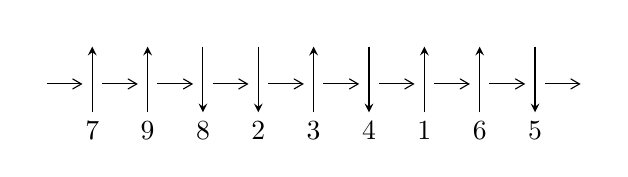
\begin{tikzpicture}[x=20pt, y=17pt]
	% nodes
	\node (C0) at (0, 0) {};
	\node (C1) at (1, 0) {};
	\node (C1U) at (1, +1) {};
	\node (C1D) at (1, -1) {7};

	\node (C2) at (2, 0) {};
	\node (C2U) at (2, +1) {};
	\node (C2D) at (2, -1) {9};

	\node (C3) at (3, 0) {};
	\node (C3U) at (3, +1) {};
	\node (C3D) at (3, -1) {8};

	\node (C4) at (4, 0) {};
	\node (C4U) at (4, +1) {};
	\node (C4D) at (4, -1) {2};

	\node (C5) at (5, 0) {};
	\node (C5U) at (5, +1) {};
	\node (C5D) at (5, -1) {3};

	\node (C6) at (6, 0) {};
	\node (C6U) at (6, +1) {};
	\node (C6D) at (6, -1) {4};

	\node (C7) at (7, 0) {};
	\node (C7U) at (7, +1) {};
	\node (C7D) at (7, -1) {1};

	\node (C8) at (8, 0) {};
	\node (C8U) at (8, +1) {};
	\node (C8D) at (8, -1) {6};

	\node (C9) at (9, 0) {};
	\node (C9U) at (9, +1) {};
	\node (C9D) at (9, -1) {5};
	\node (C10) at (10, 0) {};

	% arrows
	\draw[->,>={angle 60}]
	(C0) edge (C1) (C1) edge (C2) (C2) edge (C3) (C3) edge (C4) (C4) edge (C5) (C5) edge (C6) (C6) edge (C7) (C7) edge (C8) (C8) edge (C9) (C9) edge (C10) ;	\draw[->,>=stealth]
	(C1D) edge (C1U) (C2D) edge (C2U) (C3U) edge (C3D) (C4U) edge (C4D) (C5D) edge (C5U) (C6U) edge (C6D) (C7D) edge (C7U) (C8D) edge (C8U) (C9U) edge (C9D) ;
	\end{tikzpicture} \\
\hhline{~~} \\& 
\textbf{Solving Sequence} \\ \cline{2-2} 
 &
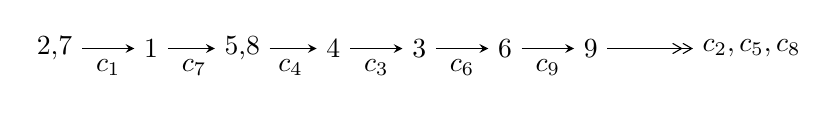
\begin{tikzpicture}[x=31pt, y=7pt]
	% node
	\node (A0) at (-1/8, 0) {2,7};
	\node (A1) at (1, 0) {1};
	\node (A2) at (33/16, 0) {5,8};
	\node (A3) at (25/8, 0) {4};
	\node (A4) at (33/8, 0) {3};
	\node (A5) at (41/8, 0) {6};
	\node (A6) at (49/8, 0) {9};
	\node (C1) at (1/2, -1) {$c_{1}$};
	\node (C2) at (3/2, -1) {$c_{7}$};
	\node (C3) at (21/8, -1) {$c_{4}$};
	\node (C4) at (29/8, -1) {$c_{3}$};
	\node (C5) at (37/8, -1) {$c_{6}$};
	\node (C6) at (45/8, -1) {$c_{9}$};
	\node (A7) at (8, 0) {$c_{2},c_{5},c_{8}$};

	% edge
	\draw[->,>=stealth]	
	(A0) edge (A1) (A1) edge (A2) (A2) edge (A3) (A3) edge (A4) (A4) edge (A5) (A5) edge (A6) ;
	\draw[->>,>={angle 60}]	
	(A6) edge (A7);
\end{tikzpicture} \\ 

\end{tabular} \\

\footnotetext{
The image of knot diagram is generated by the software ``\textbf{Draw programme}" developed by Andrew Bartholomew(\url{http://www.layer8.co.uk/maths/draw/index.htm\#Running-draw}), where we modified some parts for our purpose(\url{https://github.com/CATsTAILs/LinksPainter}).
}\phantom \\ \newline 
\centering \textbf{Ideals for irreducible components\footnotemark of $X_{\text{par}}$} 
 
\begin{align*}
I^u_{1}&=\langle 
-61 u^{16}-298 u^{15}+\cdots+43 b+351,\;-107 u^{16}-319 u^{15}+\cdots+172 a-257,\\
\phantom{I^u_{1}}&\phantom{= \langle  }u^{17}+5 u^{16}+\cdots-21 u-4\rangle \\
I^u_{2}&=\langle 
u^{10} a-2 u^9 a+\cdots+a-1,\;- u^9 a- u^{10}+\cdots+a^2+1,\\
\phantom{I^u_{2}}&\phantom{= \langle  }u^{11}-3 u^{10}+8 u^9-13 u^8+18 u^7-20 u^6+18 u^5-15 u^4+9 u^3-5 u^2+2 u-1\rangle \\
I^u_{3}&=\langle 
- u^3+2 u^2+b-2 u+1,\;u^4- u^3+a+u-2,\;u^5-2 u^4+3 u^3-3 u^2+u-1\rangle \\
\\
\end{align*}
\raggedright * 3 irreducible components of $\dim_{\mathbb{C}}=0$, with total 44 representations.\\
\footnotetext{All coefficients of polynomials are rational numbers. But the coefficients are sometimes approximated in decimal forms when there is not enough margin.}
\newpage
\renewcommand{\arraystretch}{1}
\centering \section*{I. $I^u_{1}= \langle -61 u^{16}-298 u^{15}+\cdots+43 b+351,\;-107 u^{16}-319 u^{15}+\cdots+172 a-257,\;u^{17}+5 u^{16}+\cdots-21 u-4 \rangle$}
\flushleft \textbf{(i) Arc colorings}\\
\begin{tabular}{m{7pt} m{180pt} m{7pt} m{180pt} }
\flushright $a_{2}=$&$\begin{pmatrix}1\\0\end{pmatrix}$ \\
\flushright $a_{7}=$&$\begin{pmatrix}0\\u\end{pmatrix}$ \\
\flushright $a_{1}=$&$\begin{pmatrix}1\\u^2\end{pmatrix}$ \\
\flushright $a_{5}=$&$\begin{pmatrix}0.622093 u^{16}+1.85465 u^{15}+\cdots+5.02907 u+1.49419\\1.41860 u^{16}+6.93023 u^{15}+\cdots-36.1860 u-8.16279\end{pmatrix}$ \\
\flushright $a_{8}=$&$\begin{pmatrix}u\\u^3+u\end{pmatrix}$ \\
\flushright $a_{4}=$&$\begin{pmatrix}2.04070 u^{16}+8.78488 u^{15}+\cdots-31.1570 u-6.66860\\1.41860 u^{16}+6.93023 u^{15}+\cdots-36.1860 u-8.16279\end{pmatrix}$ \\
\flushright $a_{3}=$&$\begin{pmatrix}0.901163 u^{16}+3.80814 u^{15}+\cdots-14.7616 u-2.94767\\0.720930 u^{16}+3.04651 u^{15}+\cdots-9.20930 u-1.55814\end{pmatrix}$ \\
\flushright $a_{6}=$&$\begin{pmatrix}-3.56395 u^{16}-14.4477 u^{15}+\cdots+49.8895 u+13.1221\\-3.37209 u^{16}-15.6047 u^{15}+\cdots+62.7209 u+14.2558\end{pmatrix}$ \\
\flushright $a_{9}=$&$\begin{pmatrix}-0.843023 u^{16}-4.40116 u^{15}+\cdots+26.6802 u+7.56395\\-0.604651 u^{16}-2.23256 u^{15}+\cdots+18.0465 u+5.79070\end{pmatrix}$\\ \flushright $a_{9}=$&$\begin{pmatrix}-0.843023 u^{16}-4.40116 u^{15}+\cdots+26.6802 u+7.56395\\-0.604651 u^{16}-2.23256 u^{15}+\cdots+18.0465 u+5.79070\end{pmatrix}$\\&\end{tabular}
\flushleft \textbf{(ii) Obstruction class $= -1$}\\~\\
\flushleft \textbf{(iii) Cusp Shapes $= \frac{441}{43} u^{16}+\frac{1969}{43} u^{15}+\cdots-\frac{7549}{43} u-\frac{2042}{43}$}\\~\\
\newpage\renewcommand{\arraystretch}{1}
\flushleft \textbf{(iv) u-Polynomials at the component}\newline \\
\begin{tabular}{m{50pt}|m{274pt}}
Crossings & \hspace{64pt}u-Polynomials at each crossing \\
\hline $$\begin{aligned}c_{1},c_{7}\end{aligned}$$&$\begin{aligned}
&u^{17}+5 u^{16}+\cdots-21 u-4
\end{aligned}$\\
\hline $$\begin{aligned}c_{2},c_{8}\end{aligned}$$&$\begin{aligned}
&u^{17}+u^{16}+\cdots- u-1
\end{aligned}$\\
\hline $$\begin{aligned}c_{3},c_{9}\end{aligned}$$&$\begin{aligned}
&u^{17}+5 u^{13}+\cdots+4 u-1
\end{aligned}$\\
\hline $$\begin{aligned}c_{4},c_{6}\end{aligned}$$&$\begin{aligned}
&u^{17}+2 u^{16}+\cdots+8 u-1
\end{aligned}$\\
\hline $$\begin{aligned}c_{5}\end{aligned}$$&$\begin{aligned}
&u^{17}+10 u^{16}+\cdots+5 u+2
\end{aligned}$\\
\hline
\end{tabular}\\~\\
\newpage\renewcommand{\arraystretch}{1}
\flushleft \textbf{(v) Riley Polynomials at the component}\newline \\
\begin{tabular}{m{50pt}|m{274pt}}
Crossings & \hspace{64pt}Riley Polynomials at each crossing \\
\hline $$\begin{aligned}c_{1},c_{7}\end{aligned}$$&$\begin{aligned}
&y^{17}+9 y^{16}+\cdots+17 y-16
\end{aligned}$\\
\hline $$\begin{aligned}c_{2},c_{8}\end{aligned}$$&$\begin{aligned}
&y^{17}+7 y^{16}+\cdots-19 y-1
\end{aligned}$\\
\hline $$\begin{aligned}c_{3},c_{9}\end{aligned}$$&$\begin{aligned}
&y^{17}+10 y^{15}+\cdots+10 y-1
\end{aligned}$\\
\hline $$\begin{aligned}c_{4},c_{6}\end{aligned}$$&$\begin{aligned}
&y^{17}-12 y^{16}+\cdots+46 y-1
\end{aligned}$\\
\hline $$\begin{aligned}c_{5}\end{aligned}$$&$\begin{aligned}
&y^{17}+16 y^{15}+\cdots-11 y-4
\end{aligned}$\\
\hline
\end{tabular}\\~\\
\newpage\flushleft \textbf{(vi) Complex Volumes and Cusp Shapes}
$$\begin{array}{c|c|c}  
\text{Solutions to }I^u_{1}& \I (\text{vol} + \sqrt{-1}CS) & \text{Cusp shape}\\
 \hline 
\begin{aligned}
u &= \phantom{-}0.048681 + 1.008070 I \\
a &= -1.66750 + 0.61626 I \\
b &= \phantom{-}1.134670 + 0.483593 I\end{aligned}
 & -3.35770 + 0.12402 I & -5.97884 + 0.38118 I \\ \hline\begin{aligned}
u &= \phantom{-}0.048681 - 1.008070 I \\
a &= -1.66750 - 0.61626 I \\
b &= \phantom{-}1.134670 - 0.483593 I\end{aligned}
 & -3.35770 - 0.12402 I & -5.97884 - 0.38118 I \\ \hline\begin{aligned}
u &= \phantom{-}0.423210 + 0.769632 I \\
a &= \phantom{-}0.879104 + 0.306597 I \\
b &= -0.311039 - 0.398365 I\end{aligned}
 & \phantom{-}0.28619 + 1.83578 I & \phantom{-}2.59246 - 3.36751 I \\ \hline\begin{aligned}
u &= \phantom{-}0.423210 - 0.769632 I \\
a &= \phantom{-}0.879104 - 0.306597 I \\
b &= -0.311039 + 0.398365 I\end{aligned}
 & \phantom{-}0.28619 - 1.83578 I & \phantom{-}2.59246 + 3.36751 I \\ \hline\begin{aligned}
u &= -1.115480 + 0.170377 I \\
a &= \phantom{-}0.027795 - 0.216323 I \\
b &= -0.973543 + 0.694225 I\end{aligned}
 & \phantom{-}0.27750 + 8.29795 I & \phantom{-}1.06571 - 6.88359 I \\ \hline\begin{aligned}
u &= -1.115480 - 0.170377 I \\
a &= \phantom{-}0.027795 + 0.216323 I \\
b &= -0.973543 - 0.694225 I\end{aligned}
 & \phantom{-}0.27750 - 8.29795 I & \phantom{-}1.06571 + 6.88359 I \\ \hline\begin{aligned}
u &= \phantom{-}1.18539\phantom{ +0.000000I} \\
a &= \phantom{-}0.285468\phantom{ +0.000000I} \\
b &= -0.154842\phantom{ +0.000000I}\end{aligned}
 & \phantom{-}2.39123\phantom{ +0.000000I} & \phantom{-}15.5890\phantom{ +0.000000I} \\ \hline\begin{aligned}
u &= -0.546851 + 1.063670 I \\
a &= -0.818209 + 0.890659 I \\
b &= \phantom{-}1.249560 + 0.062335 I\end{aligned}
 & -3.79067 - 2.00597 I & -6.21078 + 1.26630 I \\ \hline\begin{aligned}
u &= -0.546851 - 1.063670 I \\
a &= -0.818209 - 0.890659 I \\
b &= \phantom{-}1.249560 - 0.062335 I\end{aligned}
 & -3.79067 + 2.00597 I & -6.21078 - 1.26630 I \\ \hline\begin{aligned}
u &= -0.437546 + 1.154220 I \\
a &= -1.81788 + 0.29672 I \\
b &= \phantom{-}1.40541 + 1.07727 I\end{aligned}
 & -4.31147 - 5.61068 I & -7.96642 + 8.06049 I\\
 \hline 
 \end{array}$$\newpage$$\begin{array}{c|c|c}  
\text{Solutions to }I^u_{1}& \I (\text{vol} + \sqrt{-1}CS) & \text{Cusp shape}\\
 \hline 
\begin{aligned}
u &= -0.437546 - 1.154220 I \\
a &= -1.81788 - 0.29672 I \\
b &= \phantom{-}1.40541 - 1.07727 I\end{aligned}
 & -4.31147 + 5.61068 I & -7.96642 - 8.06049 I \\ \hline\begin{aligned}
u &= -0.582313 + 0.090917 I \\
a &= \phantom{-}0.732188 - 0.199615 I \\
b &= \phantom{-}0.842156 - 0.620975 I\end{aligned}
 & -1.32135 + 1.62186 I & -2.58195 - 4.11393 I \\ \hline\begin{aligned}
u &= -0.582313 - 0.090917 I \\
a &= \phantom{-}0.732188 + 0.199615 I \\
b &= \phantom{-}0.842156 + 0.620975 I\end{aligned}
 & -1.32135 - 1.62186 I & -2.58195 + 4.11393 I \\ \hline\begin{aligned}
u &= -0.59542 + 1.30831 I \\
a &= \phantom{-}1.58913 - 0.22054 I \\
b &= -1.40015 - 0.93567 I\end{aligned}
 & -3.3114 - 14.3446 I & -1.18187 + 8.40363 I \\ \hline\begin{aligned}
u &= -0.59542 - 1.30831 I \\
a &= \phantom{-}1.58913 + 0.22054 I \\
b &= -1.40015 + 0.93567 I\end{aligned}
 & -3.3114 + 14.3446 I & -1.18187 - 8.40363 I \\ \hline\begin{aligned}
u &= -0.28698 + 1.44004 I \\
a &= \phantom{-}0.807648 - 0.511056 I \\
b &= -0.869639 - 0.080492 I\end{aligned}
 & -5.40594 + 3.12036 I & -5.53287 - 3.71986 I \\ \hline\begin{aligned}
u &= -0.28698 - 1.44004 I \\
a &= \phantom{-}0.807648 + 0.511056 I \\
b &= -0.869639 + 0.080492 I\end{aligned}
 & -5.40594 - 3.12036 I & -5.53287 + 3.71986 I\\
 \hline 
 \end{array}$$\newpage\newpage\renewcommand{\arraystretch}{1}
\centering \section*{II. $I^u_{2}= \langle u^{10} a-2 u^9 a+\cdots+a-1,\;- u^9 a- u^{10}+\cdots+a^2+1,\;u^{11}-3 u^{10}+\cdots+2 u-1 \rangle$}
\flushleft \textbf{(i) Arc colorings}\\
\begin{tabular}{m{7pt} m{180pt} m{7pt} m{180pt} }
\flushright $a_{2}=$&$\begin{pmatrix}1\\0\end{pmatrix}$ \\
\flushright $a_{7}=$&$\begin{pmatrix}0\\u\end{pmatrix}$ \\
\flushright $a_{1}=$&$\begin{pmatrix}1\\u^2\end{pmatrix}$ \\
\flushright $a_{5}=$&$\begin{pmatrix}a\\- u^{10} a+2 u^9 a+\cdots- a+1\end{pmatrix}$ \\
\flushright $a_{8}=$&$\begin{pmatrix}u\\u^3+u\end{pmatrix}$ \\
\flushright $a_{4}=$&$\begin{pmatrix}- u^{10} a+2 u^9 a+\cdots-2 u+1\\- u^{10} a+2 u^9 a+\cdots- a+1\end{pmatrix}$ \\
\flushright $a_{3}=$&$\begin{pmatrix}u^9-2 u^8+4 u^7-3 u^6+u^5+u^3 a+u^4-4 u^3+a u+2 u^2+a-3 u+1\\u^{10} a-2 u^9 a+\cdots+a+1\end{pmatrix}$ \\
\flushright $a_{6}=$&$\begin{pmatrix}- u^9 a+u^9+\cdots- a+2\\1\end{pmatrix}$ \\
\flushright $a_{9}=$&$\begin{pmatrix}u^9-4 u^8+\cdots+a-1\\- u^{10} a+2 u^9 a+\cdots- a+1\end{pmatrix}$\\ \flushright $a_{9}=$&$\begin{pmatrix}u^9-4 u^8+\cdots+a-1\\- u^{10} a+2 u^9 a+\cdots- a+1\end{pmatrix}$\\&\end{tabular}
\flushleft \textbf{(ii) Obstruction class $= -1$}\\~\\
\flushleft \textbf{(iii) Cusp Shapes $= 4 u^{10}-4 u^9+8 u^8+4 u^7-8 u^6+12 u^5-12 u^4+4 u^3-8 u^2+2$}\\~\\
\newpage\renewcommand{\arraystretch}{1}
\flushleft \textbf{(iv) u-Polynomials at the component}\newline \\
\begin{tabular}{m{50pt}|m{274pt}}
Crossings & \hspace{64pt}u-Polynomials at each crossing \\
\hline $$\begin{aligned}c_{1},c_{7}\end{aligned}$$&$\begin{aligned}
&(u^{11}-3 u^{10}+\cdots+2 u-1)^{2}
\end{aligned}$\\
\hline $$\begin{aligned}c_{2},c_{8}\end{aligned}$$&$\begin{aligned}
&u^{22}+3 u^{21}+\cdots+6 u+1
\end{aligned}$\\
\hline $$\begin{aligned}c_{3},c_{9}\end{aligned}$$&$\begin{aligned}
&u^{22}+u^{21}+\cdots-10 u+1
\end{aligned}$\\
\hline $$\begin{aligned}c_{4},c_{6}\end{aligned}$$&$\begin{aligned}
&u^{22}- u^{21}+\cdots-4 u+1
\end{aligned}$\\
\hline $$\begin{aligned}c_{5}\end{aligned}$$&$\begin{aligned}
&(u^{11}-5 u^{10}+12 u^9-15 u^8+8 u^7+4 u^6-8 u^5+3 u^4+3 u^3-3 u^2+1)^2
\end{aligned}$\\
\hline
\end{tabular}\\~\\
\newpage\renewcommand{\arraystretch}{1}
\flushleft \textbf{(v) Riley Polynomials at the component}\newline \\
\begin{tabular}{m{50pt}|m{274pt}}
Crossings & \hspace{64pt}Riley Polynomials at each crossing \\
\hline $$\begin{aligned}c_{1},c_{7}\end{aligned}$$&$\begin{aligned}
&(y^{11}+7 y^{10}+\cdots-6 y-1)^{2}
\end{aligned}$\\
\hline $$\begin{aligned}c_{2},c_{8}\end{aligned}$$&$\begin{aligned}
&y^{22}-5 y^{21}+\cdots+72 y^2+1
\end{aligned}$\\
\hline $$\begin{aligned}c_{3},c_{9}\end{aligned}$$&$\begin{aligned}
&y^{22}- y^{21}+\cdots-8 y+1
\end{aligned}$\\
\hline $$\begin{aligned}c_{4},c_{6}\end{aligned}$$&$\begin{aligned}
&y^{22}+3 y^{21}+\cdots+8 y+1
\end{aligned}$\\
\hline $$\begin{aligned}c_{5}\end{aligned}$$&$\begin{aligned}
&(y^{11}- y^{10}+\cdots+6 y-1)^{2}
\end{aligned}$\\
\hline
\end{tabular}\\~\\
\newpage\flushleft \textbf{(vi) Complex Volumes and Cusp Shapes}
$$\begin{array}{c|c|c}  
\text{Solutions to }I^u_{2}& \I (\text{vol} + \sqrt{-1}CS) & \text{Cusp shape}\\
 \hline 
\begin{aligned}
u &= -0.253759 + 0.946686 I \\
a &= -0.049055 - 1.213920 I \\
b &= -0.33551 + 1.93421 I\end{aligned}
 & -0.13765 - 5.21629 I & \phantom{-}0.43603 + 9.01278 I \\ \hline\begin{aligned}
u &= -0.253759 + 0.946686 I \\
a &= -2.57911 - 0.36655 I \\
b &= \phantom{-}0.584301 + 0.546847 I\end{aligned}
 & -0.13765 - 5.21629 I & \phantom{-}0.43603 + 9.01278 I \\ \hline\begin{aligned}
u &= -0.253759 - 0.946686 I \\
a &= -0.049055 + 1.213920 I \\
b &= -0.33551 - 1.93421 I\end{aligned}
 & -0.13765 + 5.21629 I & \phantom{-}0.43603 - 9.01278 I \\ \hline\begin{aligned}
u &= -0.253759 - 0.946686 I \\
a &= -2.57911 + 0.36655 I \\
b &= \phantom{-}0.584301 - 0.546847 I\end{aligned}
 & -0.13765 + 5.21629 I & \phantom{-}0.43603 - 9.01278 I \\ \hline\begin{aligned}
u &= \phantom{-}1.10821\phantom{ +0.000000I} \\
a &= \phantom{-}0.305204 + 0.028042 I \\
b &= -0.160435 - 0.287182 I\end{aligned}
 & \phantom{-}2.37876\phantom{ +0.000000I} & \phantom{-}12.2610\phantom{ +0.000000I} \\ \hline\begin{aligned}
u &= \phantom{-}1.10821\phantom{ +0.000000I} \\
a &= \phantom{-}0.305204 - 0.028042 I \\
b &= -0.160435 + 0.287182 I\end{aligned}
 & \phantom{-}2.37876\phantom{ +0.000000I} & \phantom{-}12.2610\phantom{ +0.000000I} \\ \hline\begin{aligned}
u &= \phantom{-}0.572881 + 0.536287 I \\
a &= \phantom{-}0.605018 - 0.138715 I \\
b &= \phantom{-}0.379406 - 0.599968 I\end{aligned}
 & \phantom{-}0.42400 + 2.24779 I & \phantom{-}3.63582 - 5.06360 I \\ \hline\begin{aligned}
u &= \phantom{-}0.572881 + 0.536287 I \\
a &= \phantom{-}1.12964 + 0.99333 I \\
b &= -0.960104 - 0.104756 I\end{aligned}
 & \phantom{-}0.42400 + 2.24779 I & \phantom{-}3.63582 - 5.06360 I \\ \hline\begin{aligned}
u &= \phantom{-}0.572881 - 0.536287 I \\
a &= \phantom{-}0.605018 + 0.138715 I \\
b &= \phantom{-}0.379406 + 0.599968 I\end{aligned}
 & \phantom{-}0.42400 - 2.24779 I & \phantom{-}3.63582 + 5.06360 I \\ \hline\begin{aligned}
u &= \phantom{-}0.572881 - 0.536287 I \\
a &= \phantom{-}1.12964 - 0.99333 I \\
b &= -0.960104 + 0.104756 I\end{aligned}
 & \phantom{-}0.42400 - 2.24779 I & \phantom{-}3.63582 + 5.06360 I\\
 \hline 
 \end{array}$$\newpage$$\begin{array}{c|c|c}  
\text{Solutions to }I^u_{2}& \I (\text{vol} + \sqrt{-1}CS) & \text{Cusp shape}\\
 \hline 
\begin{aligned}
u &= \phantom{-}0.290349 + 1.272230 I \\
a &= \phantom{-}1.21435 + 0.88581 I \\
b &= -0.734695 + 0.377618 I\end{aligned}
 & -4.63073 + 5.00074 I & -7.84059 - 6.22751 I \\ \hline\begin{aligned}
u &= \phantom{-}0.290349 + 1.272230 I \\
a &= -1.62496 + 0.36379 I \\
b &= \phantom{-}1.46811 - 0.97707 I\end{aligned}
 & -4.63073 + 5.00074 I & -7.84059 - 6.22751 I \\ \hline\begin{aligned}
u &= \phantom{-}0.290349 - 1.272230 I \\
a &= \phantom{-}1.21435 - 0.88581 I \\
b &= -0.734695 - 0.377618 I\end{aligned}
 & -4.63073 - 5.00074 I & -7.84059 + 6.22751 I \\ \hline\begin{aligned}
u &= \phantom{-}0.290349 - 1.272230 I \\
a &= -1.62496 - 0.36379 I \\
b &= \phantom{-}1.46811 + 0.97707 I\end{aligned}
 & -4.63073 - 5.00074 I & -7.84059 + 6.22751 I \\ \hline\begin{aligned}
u &= -0.234018 + 0.605151 I \\
a &= \phantom{-}0.357585 - 0.648167 I \\
b &= \phantom{-}0.378854 - 1.068730 I\end{aligned}
 & \phantom{-}0.80290 + 2.70441 I & \phantom{-}3.46762 + 0.08333 I \\ \hline\begin{aligned}
u &= -0.234018 + 0.605151 I \\
a &= \phantom{-}2.61356 + 0.79794 I \\
b &= -0.866642 - 0.847442 I\end{aligned}
 & \phantom{-}0.80290 + 2.70441 I & \phantom{-}3.46762 + 0.08333 I \\ \hline\begin{aligned}
u &= -0.234018 - 0.605151 I \\
a &= \phantom{-}0.357585 + 0.648167 I \\
b &= \phantom{-}0.378854 + 1.068730 I\end{aligned}
 & \phantom{-}0.80290 - 2.70441 I & \phantom{-}3.46762 - 0.08333 I \\ \hline\begin{aligned}
u &= -0.234018 - 0.605151 I \\
a &= \phantom{-}2.61356 - 0.79794 I \\
b &= -0.866642 + 0.847442 I\end{aligned}
 & \phantom{-}0.80290 - 2.70441 I & \phantom{-}3.46762 - 0.08333 I \\ \hline\begin{aligned}
u &= \phantom{-}0.57044 + 1.34258 I \\
a &= -0.862107 + 0.035474 I \\
b &= \phantom{-}0.818255 - 0.852218 I\end{aligned}
 & -1.76023 + 5.92443 I & \phantom{-}3.17045 - 10.02355 I \\ \hline\begin{aligned}
u &= \phantom{-}0.57044 + 1.34258 I \\
a &= \phantom{-}1.389870 + 0.219943 I \\
b &= -1.071530 + 0.524779 I\end{aligned}
 & -1.76023 + 5.92443 I & \phantom{-}3.17045 - 10.02355 I\\
 \hline 
 \end{array}$$\newpage$$\begin{array}{c|c|c}  
\text{Solutions to }I^u_{2}& \I (\text{vol} + \sqrt{-1}CS) & \text{Cusp shape}\\
 \hline 
\begin{aligned}
u &= \phantom{-}0.57044 - 1.34258 I \\
a &= -0.862107 - 0.035474 I \\
b &= \phantom{-}0.818255 + 0.852218 I\end{aligned}
 & -1.76023 - 5.92443 I & \phantom{-}3.17045 + 10.02355 I \\ \hline\begin{aligned}
u &= \phantom{-}0.57044 - 1.34258 I \\
a &= \phantom{-}1.389870 - 0.219943 I \\
b &= -1.071530 - 0.524779 I\end{aligned}
 & -1.76023 - 5.92443 I & \phantom{-}3.17045 + 10.02355 I\\
 \hline 
 \end{array}$$\newpage\newpage\renewcommand{\arraystretch}{1}
\centering \section*{III. $I^u_{3}= \langle - u^3+2 u^2+b-2 u+1,\;u^4- u^3+a+u-2,\;u^5-2 u^4+3 u^3-3 u^2+u-1 \rangle$}
\flushleft \textbf{(i) Arc colorings}\\
\begin{tabular}{m{7pt} m{180pt} m{7pt} m{180pt} }
\flushright $a_{2}=$&$\begin{pmatrix}1\\0\end{pmatrix}$ \\
\flushright $a_{7}=$&$\begin{pmatrix}0\\u\end{pmatrix}$ \\
\flushright $a_{1}=$&$\begin{pmatrix}1\\u^2\end{pmatrix}$ \\
\flushright $a_{5}=$&$\begin{pmatrix}- u^4+u^3- u+2\\u^3-2 u^2+2 u-1\end{pmatrix}$ \\
\flushright $a_{8}=$&$\begin{pmatrix}u\\u^3+u\end{pmatrix}$ \\
\flushright $a_{4}=$&$\begin{pmatrix}- u^4+2 u^3-2 u^2+u+1\\u^3-2 u^2+2 u-1\end{pmatrix}$ \\
\flushright $a_{3}=$&$\begin{pmatrix}- u^4+u^3- u^2+2\\- u^4+2 u^3-3 u^2+2 u-1\end{pmatrix}$ \\
\flushright $a_{6}=$&$\begin{pmatrix}- u^4+3 u^3-4 u^2+4 u-2\\u^4- u^3+u^2-1\end{pmatrix}$ \\
\flushright $a_{9}=$&$\begin{pmatrix}u^4-2 u^3+3 u^2-2 u\\u^2- u+1\end{pmatrix}$\\ \flushright $a_{9}=$&$\begin{pmatrix}u^4-2 u^3+3 u^2-2 u\\u^2- u+1\end{pmatrix}$\\&\end{tabular}
\flushleft \textbf{(ii) Obstruction class $= 1$}\\~\\
\flushleft \textbf{(iii) Cusp Shapes $= -6 u^4+13 u^3-22 u^2+14 u-9$}\\~\\
\newpage\renewcommand{\arraystretch}{1}
\flushleft \textbf{(iv) u-Polynomials at the component}\newline \\
\begin{tabular}{m{50pt}|m{274pt}}
Crossings & \hspace{64pt}u-Polynomials at each crossing \\
\hline $$\begin{aligned}c_{1}\end{aligned}$$&$\begin{aligned}
&u^5-2 u^4+3 u^3-3 u^2+u-1
\end{aligned}$\\
\hline $$\begin{aligned}c_{2},c_{8}\end{aligned}$$&$\begin{aligned}
&u^5- u^4- u^3+u^2-1
\end{aligned}$\\
\hline $$\begin{aligned}c_{3},c_{9}\end{aligned}$$&$\begin{aligned}
&u^5- u^3+u^2+u-1
\end{aligned}$\\
\hline $$\begin{aligned}c_{4},c_{6}\end{aligned}$$&$\begin{aligned}
&u^5+2 u^4+3 u^3+3 u^2+3 u+1
\end{aligned}$\\
\hline $$\begin{aligned}c_{5}\end{aligned}$$&$\begin{aligned}
&u^5-3 u^4+5 u^3-4 u^2+3 u-1
\end{aligned}$\\
\hline $$\begin{aligned}c_{7}\end{aligned}$$&$\begin{aligned}
&u^5+2 u^4+3 u^3+3 u^2+u+1
\end{aligned}$\\
\hline
\end{tabular}\\~\\
\newpage\renewcommand{\arraystretch}{1}
\flushleft \textbf{(v) Riley Polynomials at the component}\newline \\
\begin{tabular}{m{50pt}|m{274pt}}
Crossings & \hspace{64pt}Riley Polynomials at each crossing \\
\hline $$\begin{aligned}c_{1},c_{7}\end{aligned}$$&$\begin{aligned}
&y^5+2 y^4- y^3-7 y^2-5 y-1
\end{aligned}$\\
\hline $$\begin{aligned}c_{2},c_{8}\end{aligned}$$&$\begin{aligned}
&y^5-3 y^4+3 y^3-3 y^2+2 y-1
\end{aligned}$\\
\hline $$\begin{aligned}c_{3},c_{9}\end{aligned}$$&$\begin{aligned}
&y^5-2 y^4+3 y^3-3 y^2+3 y-1
\end{aligned}$\\
\hline $$\begin{aligned}c_{4},c_{6}\end{aligned}$$&$\begin{aligned}
&y^5+2 y^4+3 y^3+5 y^2+3 y-1
\end{aligned}$\\
\hline $$\begin{aligned}c_{5}\end{aligned}$$&$\begin{aligned}
&y^5+y^4+7 y^3+8 y^2+y-1
\end{aligned}$\\
\hline
\end{tabular}\\~\\
\newpage\flushleft \textbf{(vi) Complex Volumes and Cusp Shapes}
$$\begin{array}{c|c|c}  
\text{Solutions to }I^u_{3}& \I (\text{vol} + \sqrt{-1}CS) & \text{Cusp shape}\\
 \hline 
\begin{aligned}
u &= \phantom{-}0.372466 + 1.263920 I \\
a &= -1.347300 - 0.010044 I \\
b &= \phantom{-}0.929085 - 0.848284 I\end{aligned}
 & -3.01018 + 5.17259 I & -1.67537 - 5.94701 I \\ \hline\begin{aligned}
u &= \phantom{-}0.372466 - 1.263920 I \\
a &= -1.347300 + 0.010044 I \\
b &= \phantom{-}0.929085 + 0.848284 I\end{aligned}
 & -3.01018 - 5.17259 I & -1.67537 + 5.94701 I \\ \hline\begin{aligned}
u &= \phantom{-}1.33263\phantom{ +0.000000I} \\
a &= -0.119827\phantom{ +0.000000I} \\
b &= \phantom{-}0.480071\phantom{ +0.000000I}\end{aligned}
 & \phantom{-}2.14584\phantom{ +0.000000I} & -17.5700\phantom{ +0.000000I} \\ \hline\begin{aligned}
u &= -0.038780 + 0.656277 I \\
a &= \phantom{-}1.90721 - 0.97967 I \\
b &= -0.169121 + 1.134660 I\end{aligned}
 & \phantom{-}0.29233 - 3.70382 I & -0.53969 + 6.40947 I \\ \hline\begin{aligned}
u &= -0.038780 - 0.656277 I \\
a &= \phantom{-}1.90721 + 0.97967 I \\
b &= -0.169121 - 1.134660 I\end{aligned}
 & \phantom{-}0.29233 + 3.70382 I & -0.53969 - 6.40947 I\\
 \hline 
 \end{array}$$\newpage
\newpage\renewcommand{\arraystretch}{1}
\centering \section*{ IV. u-Polynomials}
\begin{tabular}{m{50pt}|m{274pt}}
Crossings & \hspace{64pt}u-Polynomials at each crossing \\
\hline $$\begin{aligned}c_{1}\end{aligned}$$&$\begin{aligned}
&(u^5-2 u^4+3 u^3-3 u^2+u-1)(u^{11}-3 u^{10}+\cdots+2 u-1)^{2}\\
&\cdot(u^{17}+5 u^{16}+\cdots-21 u-4)
\end{aligned}$\\
\hline $$\begin{aligned}c_{2},c_{8}\end{aligned}$$&$\begin{aligned}
&(u^5- u^4- u^3+u^2-1)(u^{17}+u^{16}+\cdots- u-1)(u^{22}+3 u^{21}+\cdots+6 u+1)
\end{aligned}$\\
\hline $$\begin{aligned}c_{3},c_{9}\end{aligned}$$&$\begin{aligned}
&(u^5- u^3+u^2+u-1)(u^{17}+5 u^{13}+\cdots+4 u-1)\\
&\cdot(u^{22}+u^{21}+\cdots-10 u+1)
\end{aligned}$\\
\hline $$\begin{aligned}c_{4},c_{6}\end{aligned}$$&$\begin{aligned}
&(u^5+2 u^4+3 u^3+3 u^2+3 u+1)(u^{17}+2 u^{16}+\cdots+8 u-1)\\
&\cdot(u^{22}- u^{21}+\cdots-4 u+1)
\end{aligned}$\\
\hline $$\begin{aligned}c_{5}\end{aligned}$$&$\begin{aligned}
&(u^5-3 u^4+5 u^3-4 u^2+3 u-1)\\
&\cdot(u^{11}-5 u^{10}+12 u^9-15 u^8+8 u^7+4 u^6-8 u^5+3 u^4+3 u^3-3 u^2+1)^2\\
&\cdot(u^{17}+10 u^{16}+\cdots+5 u+2)
\end{aligned}$\\
\hline $$\begin{aligned}c_{7}\end{aligned}$$&$\begin{aligned}
&(u^5+2 u^4+3 u^3+3 u^2+u+1)(u^{11}-3 u^{10}+\cdots+2 u-1)^{2}\\
&\cdot(u^{17}+5 u^{16}+\cdots-21 u-4)
\end{aligned}$\\
\hline
\end{tabular}\newpage\renewcommand{\arraystretch}{1}
\centering \section*{ V. Riley Polynomials}
\begin{tabular}{m{50pt}|m{274pt}}
Crossings & \hspace{64pt}Riley Polynomials at each crossing \\
\hline $$\begin{aligned}c_{1},c_{7}\end{aligned}$$&$\begin{aligned}
&(y^5+2 y^4- y^3-7 y^2-5 y-1)(y^{11}+7 y^{10}+\cdots-6 y-1)^{2}\\
&\cdot(y^{17}+9 y^{16}+\cdots+17 y-16)
\end{aligned}$\\
\hline $$\begin{aligned}c_{2},c_{8}\end{aligned}$$&$\begin{aligned}
&(y^5-3 y^4+3 y^3-3 y^2+2 y-1)(y^{17}+7 y^{16}+\cdots-19 y-1)\\
&\cdot(y^{22}-5 y^{21}+\cdots+72 y^2+1)
\end{aligned}$\\
\hline $$\begin{aligned}c_{3},c_{9}\end{aligned}$$&$\begin{aligned}
&(y^5-2 y^4+3 y^3-3 y^2+3 y-1)(y^{17}+10 y^{15}+\cdots+10 y-1)\\
&\cdot(y^{22}- y^{21}+\cdots-8 y+1)
\end{aligned}$\\
\hline $$\begin{aligned}c_{4},c_{6}\end{aligned}$$&$\begin{aligned}
&(y^5+2 y^4+3 y^3+5 y^2+3 y-1)(y^{17}-12 y^{16}+\cdots+46 y-1)\\
&\cdot(y^{22}+3 y^{21}+\cdots+8 y+1)
\end{aligned}$\\
\hline $$\begin{aligned}c_{5}\end{aligned}$$&$\begin{aligned}
&(y^5+y^4+7 y^3+8 y^2+y-1)(y^{11}- y^{10}+\cdots+6 y-1)^{2}\\
&\cdot(y^{17}+16 y^{15}+\cdots-11 y-4)
\end{aligned}$\\
\hline
\end{tabular}
\vskip 2pc
\end{document}